\subsection{A Common Perspective on Enterprise Architecture}
While there is no singular agreed-upon definition for EA, different definitions\cite{jungle2004,GartnerInc,ross2006,pearlson2009,lankhorst2009,sessions2007,togaf9.1} do have much in common. EA is a discipline that takes a holistic, design-oriented approach to transforming high-level business vision and goals into the integration of an enterprise's organizational structure, business processes, and information systems. This transformation involves identifying and implementing the necessary change for this to occur. In order to view different Enterprise Architectures from a common perspective, this paper will break the frameworks down into three separate components: the EA method, the EA description, and the EA engine. 

The Method aims to lay the groundwork for the EA project. Typically, this involves setting up teams, ownership, responsibilities and gaining commitment. Also it defines the overall process of collecting, validating and approving the EA artifacts  (eg. descriptions As-Is, To-Be, gap analysis,  principles) that will form the second component - The EA description.  The Engine involves setting up a support structure for ensuring the ongoing adoption of the to-be EA description. This can involve gaining commitment from stakeholders, setting up some compliance checking procedures, and deciding upon a prioritization of tasks to be completed. The remainder of this section will look at three different EA frameworks from the perspective of of these three phases: The Open Group Architecture Framework (TOGAF), the Zachman Framework, and the Federal Enterprise Architecture (FEA)

\subsection{TOGAF}
The Open Group Architecture Framework, more commonly know as TOGAF, is a freely available EA framework created by The Open Group\footnote{~\url{www.opengroup.org}}, a consortium of IT organizations. TOGAF is comprised of a number of different aspects, mainly: the Architecture Development Method (ADM), "a method for developing and managing the lifecycle of an enterprise architecture"~\cite[Ch. 5.1]{togaf9.1}; the Architecture Content Framework, a companion to the ADM which describes the content of the products of the ADM; and the Enterprise Continuum, which provides a means to organize the produced architectures. 
\subsubsection{EA Method}
The TOGAF ADM falls under our EA Method component of EA. The TOGAF ADM is made up of a preliminary phase, six core phases (labeled A-H), and a requirements management component. 

\begin{figure}
\centering
\includegraphics[scale=0.7]{ADM}
\caption{TOGAF: ADM basic structure from \cite[Ch. 5.2.2]{togaf9.1}}
\label{fig:ADM}
\end{figure}

In TOGAF, the preliminary phase lays the groundwork for the rest of the EA process. Some important aspects are to set up a governance structure and EA team for the EA process and to establish a repository for storing all architectural information~\cite[Ch. 6]{togaf9.1}.

Phase A of the TOGAF Process, the architectural vision phase, is aimed at setting a clear vision for the enterprises future architecture. This involves creating the initial as-is architecture as well as setting clear, management approved goals and requirements, and transforming them into a high-level vision of the enterprises to-be architecture~\cite[Ch. 7]{togaf9.1}.

At this point, TOGAF suggests that the outputs of the preliminary phase and phase A be organized into a "Statement of Architecture Work". This document is to be approved by project sponsors~\cite[Ch. 7.4.11]{togaf9.1} and can be used to form the basis of a contract between the architecture provider and the client~\cite[Ch. 36.2.20]{togaf9.1}.

The next three phases, B-D are concerned with creating the as-is and to-be business architecture, information systems architecture, and the technology architecture. TOGAF suggests two different approaches to creating the architectures: baseline first or target first~\cite[Ch. 19.4]{togaf9.1}. Baseline-first involves analyzing the as-is architecture for areas where improvements can be made. Target-first aims at creating a detailed target architecture and then mapping it back to the as-is architecture in order figure out what needs to change. The main aspects of these phases are to develop the as-is and to-be architectures, analyze the gap between them, and create an initial road-map of the steps needed to cross the gap.

Phase E and F, Opportunities and Solutions and Migration Planning, are concerned with organizing the work to be done into projects, and then creating a schedule for executing the projects~\cite[Ch. 13-14]{togaf9.1}.

The final ADM phase, phase G, is concerned with the implementation and setting up a framework for its governance and its compliance to the target architecture~\cite[Ch. 15]{togaf9.1}.

\subsubsection{EA Description}
TOGAF views architecture from the perspective of four different architecture domains~\cite{sessions2007}: business, application, data, and technical. Business architecture is concerned with processes and functions used to meet business goals, application architecture is concerned with the design of specific applications and their interactions, data architecture is concerned with managing enterprise data, and the technical architecture is concerned with the infrastructure (hardware and software) used to support the applications. The architectures in these four domains are created through the ADM phases B (Business Architecture Phase), C (Information Systems Architectures Phase) and D (Technology Architecture).

The various architectural artifacts in TOGAF are organized across an Architectural Landscape~\cite[Ch. 20.2]{togaf9.1} of three dimensions: breadth, level, and time. Breadth refers to the area of subject matter for an architecture. Levels refer to the level of detail of an architecture. TOGAF specifies three levels of detail: strategic, for overall direction setting at the executive level; segment, for architectures at the level of a program or portfolio; and capability, for architectures concerned with how the architecture process is itself enabled and governed. The time dimension of the landscape keeps the state of architectures as they evolve over time. Additionally, the Architecture Landscape can be partitioned into independent partitions for supporting different organizational units~\cite[Ch. 40]{togaf9.1}. 

%Breadth: The breadth (subject matter) area is generally the primar y organizing character istic for descr ibing an Architecture Landscape. Architectures are functionally decomposed into a hierarchy of specific subject areas or segments.

%Capability Architecture provides an organizing framework for change activity and the development of effective architecture roadmaps realizing capability increments.


At each level of the Architecture Landscape, architectures are further organized through the Enterprise Continuum which provides a way to organize the architectures from generic to organization-specific~\cite[Ch. 39]{togaf9.1}. The most generic are called Foundation Architectures~\cite[Ch. 39.4.1]{togaf9.1}, which are applicable to all enterprises. A core aspect of a Foundation Architecture is to provide a high-level taxonomy which can provide a basis for the more specific architectures~\cite[Ch. 43]{togaf9.1}. TOGAF includes a Foundation Architecture which can be used, called the Technical Reference Model(TRM). The second set of architectures in the continuum are called the Common Systems Architectures~\cite[Ch. 39.4.1]{togaf9.1}. These architectures are specific to a generic problem domain (e.g. security management), and are thus applicable to a wide range (but not all) of enterprises. TOGAF includes a Common System Architecture for the domain of information integration, called the Integrated Information Infrastructure Reference Model (III-RM). The third set of architectures in the continuum are called Industry Architectures. These architectures are applicable to a specific problem within a specific industry. They are thus useful to many members of that industry, but not necessarily outside of it. The most specific level in the continuum are Organization-Specific  architectures. As the name implies, they are relevant only to a specific enterprise. These outline the architectural solution for a particular enterprise and provide "a means to communicate and manage business operations across all four architectural domains"~\cite[Ch. 39.4.1]{togaf9.1}.

%The content of TOGAF architecture artifacts is defined in the Content Framework... [Still don't really understand this part] [maybe content is actually determined through reference models which are placed on the continuum?]

% architecture landscape
% architecture partitioning
% architecture capability
% interop of partitions "federated architectures independently developed, maintained, and managed architectures that are subsequently integrated within an integration framework are typical



\subsubsection{EA Engine}

TOGAF outlines an ADM phase concerned with the ongoing change management process for the architecture of an enterprise.  It is concerned with managing changes to the architecture throughout its lifecycle~\cite[Ch. 16]{togaf9.1}. In this phase, a governance body sets criteria for determining if a change requires an architecture update if a new cycle of the ADM needs to be started. An important aspect of this process is to deploy tools for monitoring for business and technological changes and measuring performance indicators. 

TOGAF describes a formal review process for determining compliance. The main goal of this process is to "[f]irst and foremost, catch errors in the project architecture early, and thereby reduce the cost and risk of changes required later in the lifecycle"~\cite[Ch. 48.3.1]{togaf9.1}.

%\begin{figure}
%\centering
%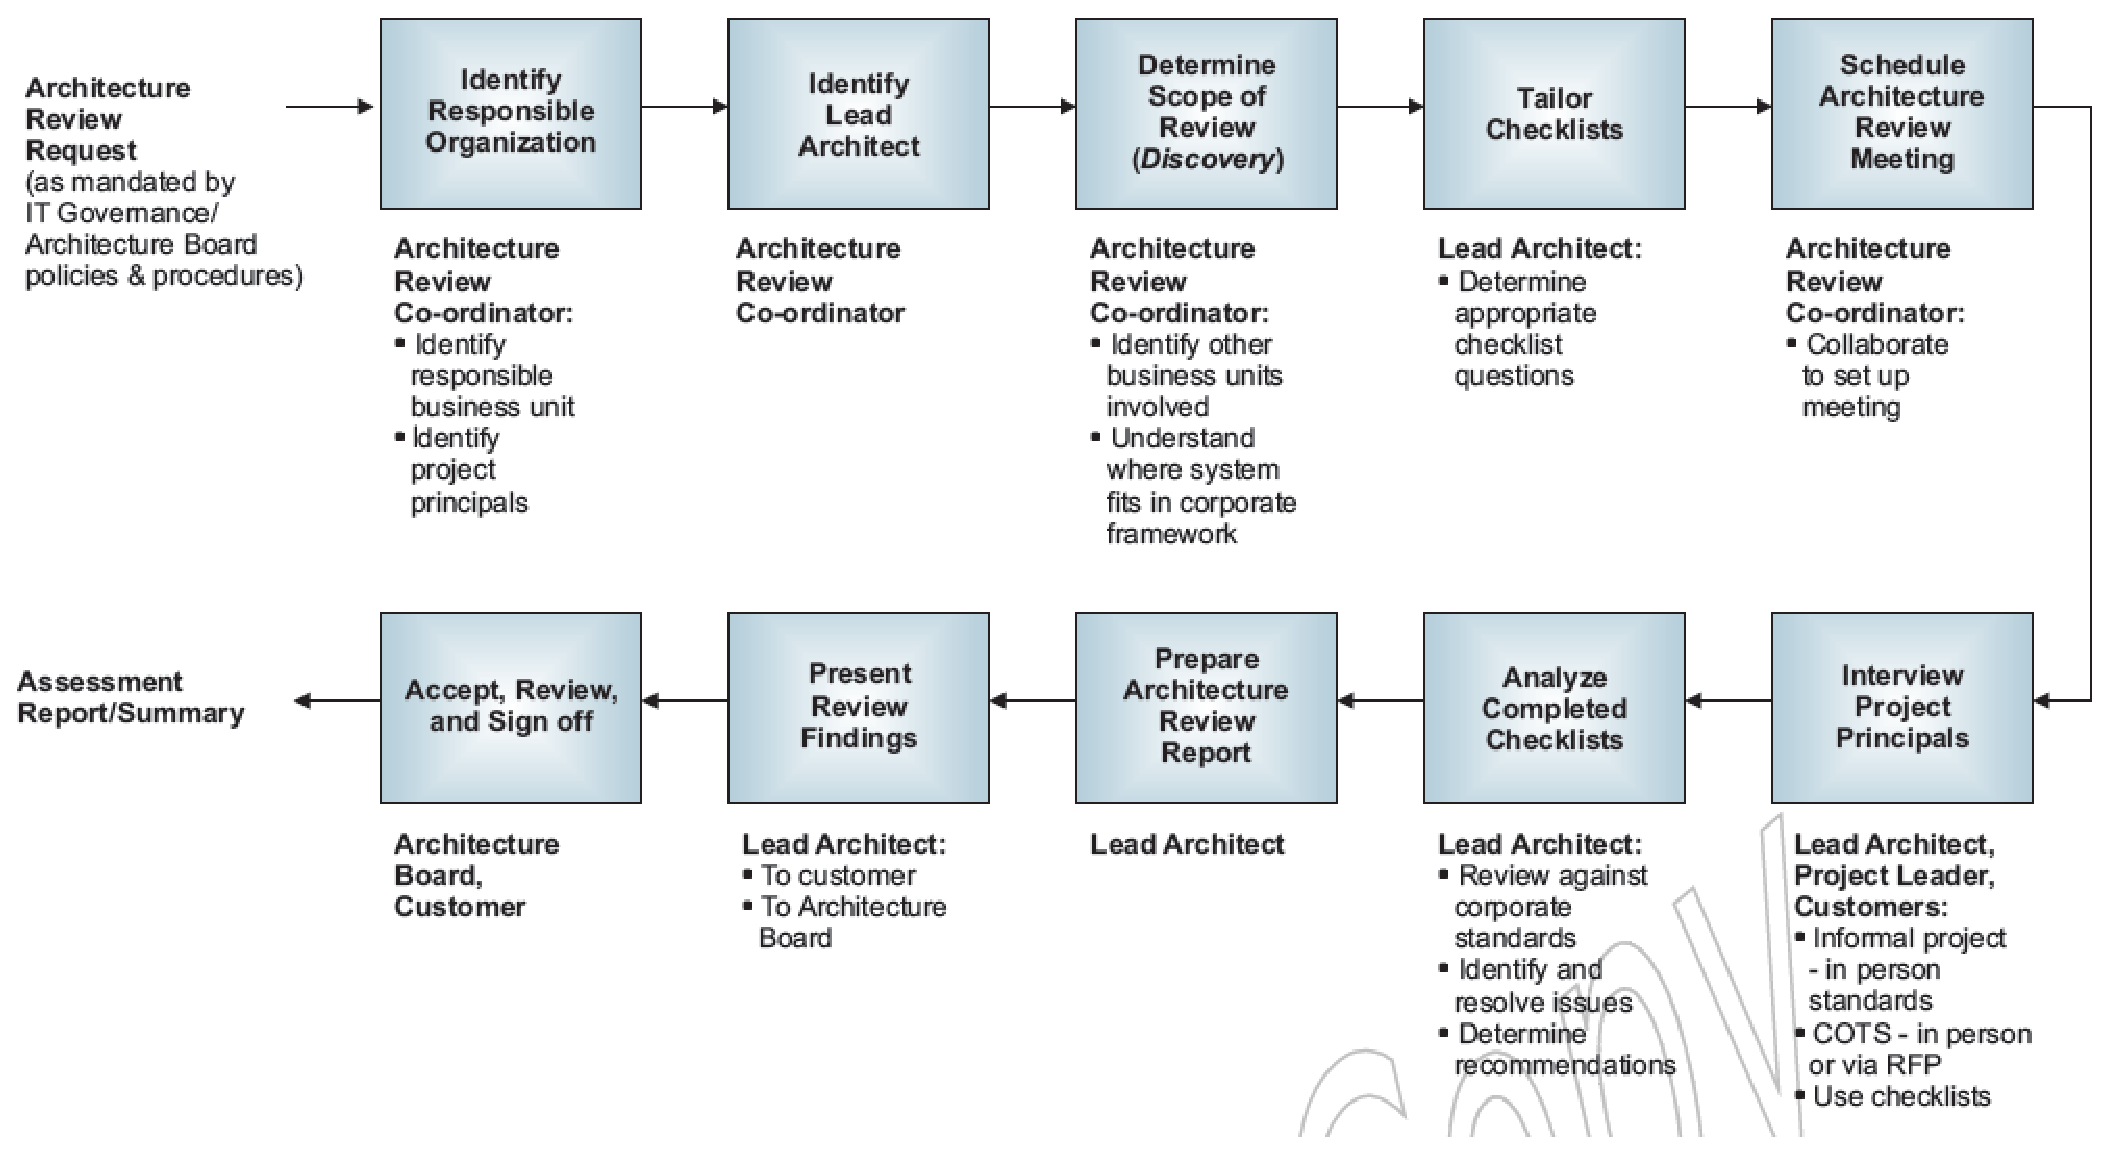
\includegraphics[scale=0.2]{togaf_compliance}
%\caption{TOGAF: Architecture Compliance Review Process from \cite[Ch. 48.4.1]{togaf9.1}}
%\label{fig:togaf_review}
%\end{figure}

%Some other goals of this process are to "Ensure the application of best practices to architecture work" "Provide an overview of the compliance of an architecture to mandated enterpr ise standards." "Identify where the standards themselves may require modification." "Communicate to management the status of technical readiness of the project." "Identify and communicate significant architectural gaps to product and service providers"

TOGAF outlines a formal approach to architecture governance which involves the setting up of an "Architecture Board to oversee the implementation of the [architecture] strategy"~\cite[Ch. 47.1]{togaf9.1}. This board has an important role in Architecture Governance, such as "[p]roviding the basis for all decision-making with regard to the architectures"~\cite[Ch. 47.2]{togaf9.1} and enforcing architecture compliance. The TOGAF Architecture Governance Framework~\cite[Ch. 50]{togaf9.1} suggests guidelines for developing a formal governance structure for the Enterprise Continuum (and thus, all the architectural artifacts) and architecture processes. 


%governance p 590

%[Repository]
%
%[requirements management]

\subsection{Zachman}
The Zachman Framework was the first EA, first introduced by John Zachman in 1987~\cite{sessions2007,zachman}. It consists only of a taxonomy, and as such only fits into the EA Description aspect of EA. 

\subsubsection{EA Description}

The Zachman Framework breaks down EA into a grid of perspectives. Each perspective is characterized by two things; its target audience and the issue is aimed at. ZF covers six issues: What (data and entities), How (functional), Where (locations and interconnections/networks), Who (people relationships), When (events and performance criteria), Why (motivations and goals)~\cite{jungle2004}. For each issue, it views it from six different perspectives: executive, business management, architect, engineer, technician, and enterprise users. 

The executive perspective is meant for executives or planners and needs to provide an estimate of a system's functionality and cost~\cite{jungle2004}. The business management perspective is a business view of how an owner thinks the business operates~\cite{Zachman2000}. The architect perspective takes a systems viewpoint and describes the operations and interactions of the variety of systems in an enterprise. The engineer perspective views describes the physical technology and design of the individual systems. The technician perspective takes the perspective of a "sub-contractor" who is implementing a specific system and the high, out-of-context level of detail associated with that. The enterprise users perspective describes the perspective of the system users. 
 
%[XXXX Zachman Diagram XXXX]


\subsection{FEA}
The Federal Enterprise Architecture (FEA)is an effort by the federal government of the United States to create an EA for the entire government. The FEA is a complete EA framework, covering all three components of EA. The Federal Enterprise Architecture Program Management Office describes FEA as "...a common language and framework to describe and analyze IT investments, enhance collaboration and ultimately transform the Federal government into a citizen-centered, results-oriented, and market-based organization as set forth in the President's Management Agenda."~\cite{FEA_PMO2007} FEA takes takes an approach where individual organizational units develop their own architectures that fit into an overall framework of common standards and interoperability.

FEA is composed of six core elements~\cite{sessions2007}:
\begin{itemize}
    \item The organization is broken-down into different segments of varying scopes, and architecture is developed for each segment
    \item A set of five reference models which are used as a basis to describe the important elements of the FEA in a consistent manner
    \item A process for creating each segment EA
    \item A transitional process for moving from the current state of the enterprise to the visioned state
    \item A taxonomy for organizing the various assets of the FEA
    \item Guidelines for measuring the degree of success of the FEA
\end{itemize}
Compared to TOGAF and Zachman Framework, FEA defines both the taxonomy for EA artifacts (EA description in Fig. \ref{fig:EA_general}) and the EA process for creating these artifacts and using them by organization (EA method and EA engine in Fig.\ref{fig:EA_general}). 

\subsubsection{EA Description}
% ~\cite{sessions2007}
FEA develops architecture for segments and enterprise services. A segment is a "major line-of-business functionality"~\cite{sessions2007} for an individual organizational unit (such as an agency or department). Two types of segments exist: core mission-area segments and business service segments~\cite{FEA_PMO2007}. Core mission-area segments are at the scope of a single organizational unit (though they may be shared by different units) and are essential to its purpose~\cite{sessions2007,FEA_PMO2007}. Business service segments are also at the scope of an individual organizational unit, however these segments exist in all organizational units and are defined for the entire enterprise. Like business service segments, enterprise services are defined organization-wide. However, they are different in that they also function at the enterprise level, e.g. a single security management service that is shared by the entire enterprise. 

The EA artifacts defined by FEA include  baseline segment architectures, target segment architectures and transition strategy. The EA transition strategy describes the overall plan and schedule to achieve the target (“to-be”) architecture.

%Segment identification is a continuous, iterative process. Enterprise assets including systems and IT investments are mapped to the agency-level reference models to create a segment-oriented view of the enterprise (see Figure 2-2). 
%
%"The FEA consists of a set of interrelated "reference models" designed to facilitate cross-agency analysis and the identification of duplicative investments, gaps, and opportunities for collaboration within and across agencies. Collectively, the reference models [compose] a framework for describing important elements of the FEA in a common and consistent way."~\cite{FederalEnterpriseArchitectureProgramManagementOffice}
%
%"This, in a nutshell, is the goal of the five FEA reference models: to give standard terms and definitions for the domains of enterprise architecture and, thereby, facilitate collaboration and sharing across the federal government."

In order to have a common language for describing the enterprises assets, FEA describes five reference models for mapping assets to segments and enterprise services~\cite{FEA_PMO2007}. The five reference models are the performance reference model, the business reference model, the service component reference model, the technical reference model, and the data reference model. 
\begin{figure}
\centering
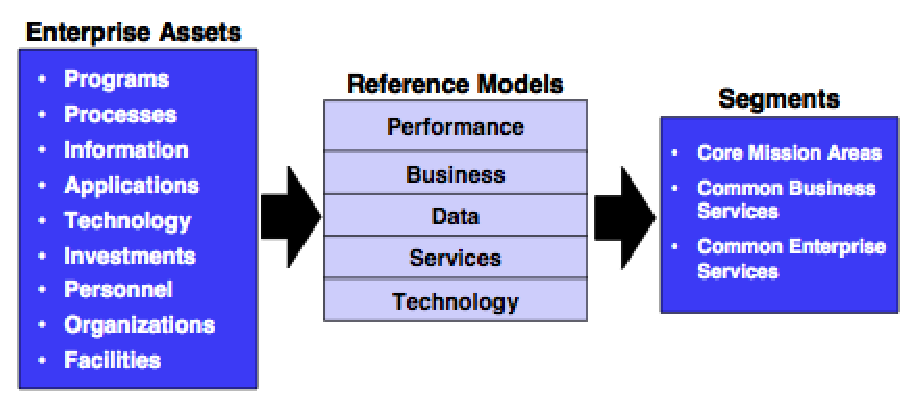
\includegraphics[scale=0.6]{FEAsegm}
\caption{FEA: Segment Identification from ~\cite{FEA_PMO2007}}
\label{fig:FEA_segmentID}
\end{figure}
%[Insert Segment Identification Figure (2.2 on page 20 of ~\cite{FederalEnterpriseArchitectureProgramManagementOffice})]

The performance reference model provides a framework for developing consistent measurement. The business reference model provides a framework for developing a functional view of the enterprises line of business. The service component reference model provides a framework for describing how the services offered by IT systems support business functionality.  The data reference model provides a framework for describing data in a consistent way that enables enterprise-wide sharing. 

\subsubsection{EA Method}

% Performance Improvement Lifecyle seems to be the overall FEA process

%"single agency contains both core mission area segments and business service segments. Enterprise services are those cross-cutting services spanning multiple segments."\cite{FederalEnterpriseArchitectureProgramManagementOffice2007}
%"By contrast, segment architecture defines a simple roadmap for a core mission area, business service or enterprise service"~\cite{FederalEnterpriseArchitectureProgramManagementOffice2007}
%
% ~\cite{sessions2007}
%
%Segments 
% - segment is a major line-of-business functionality, e.g. HR
%     - core mission-area segments, central to mission/purpose of organization
%     - business-services segment, foundational to all organizations
% - function at agency level, defined at enterprise level

% Just as enterprises are themselves hierarchically organized, so are the different views provided by each type of architecture.
 
FEA defines a four step iterative process for creating architectures for each segment and service~\cite{FEA_PMO2007}:
\begin{enumerate}
    \item Architectural analysis
    \item Architectural definition
    \item Investment and funding strategy
    \item Program management plan and execute projects
\end{enumerate}

%New and revised business and information requirements are continuously identified as the segment moves though each lifecycle phase, and as business and information management solutions are funded and developed to meet stakeholder requirements. Consequently, segment architecture work products must be maintained to reflect these inputs.

The first step, architectural analysis, is concerned with defining the scope of the segment, its baseline architecture, current problems in the segment, and a high-level vision of the desired final state for the segment~\cite{FEA_PMO2007}.

The second step, architectural definition, is concerned with defining the detailed target architecture of the segment~\cite{FEA_PMO2007}. Aside for the architecture itself, it is also necessary to define a roadmap of projects to get there, the segment transition strategy, and the performance goals of the architecture. 
  
The third step, the investment and funding strategy, is concerned with specifying how the projects identified in the segment transition strategy are to be funded~\cite{FEA_PMO2007}. 

The fourth step, program management plan and execute strategies, is concerned with making detailed plans for the individual projects, executing the plans, and defining performance measurements for the initiative~\cite{FEA_PMO2007}.
\begin{figure}
\centering
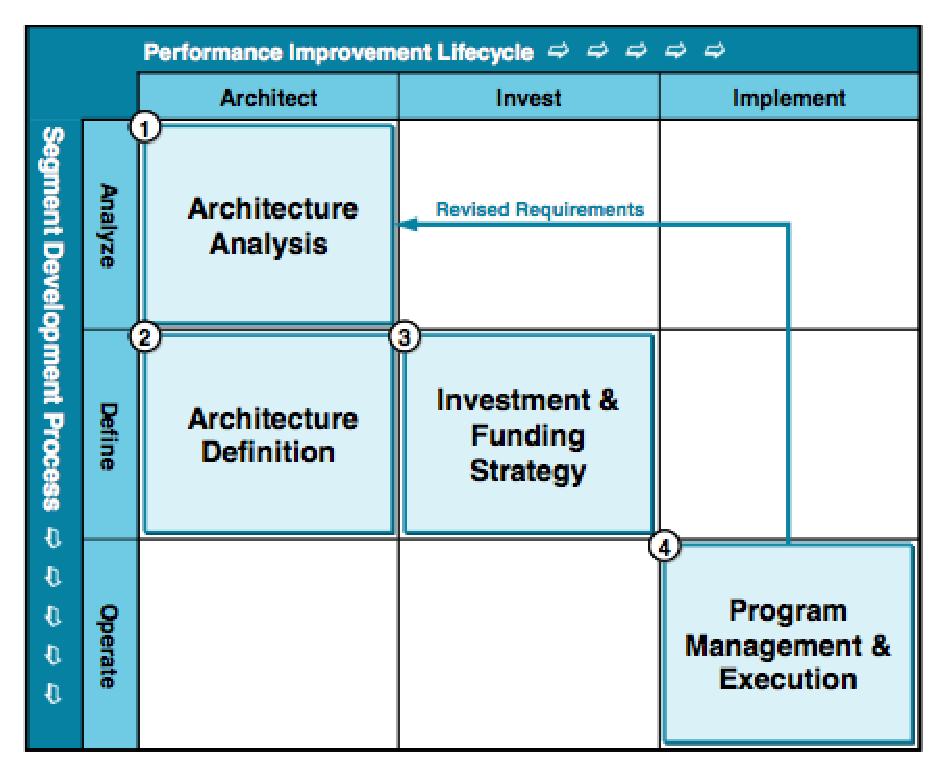
\includegraphics[scale=0.4]{FEA}
\caption{FEA: Segment Architecture Development and Maintenance from ~\cite{FEA_PMO2007}}
\label{fig:FEA_segmentDev}
\end{figure}
%[Insert Figure 3-2: Segment Architecture Development and Maintenance from ~\cite{FEA_PMO2007}]

% is there an EA agency???
    
\subsubsection{EA Engine}
%~\cite{sessions2007}

FEA describes an "engine" to maintain the architecture in order ensure that it stays relevant over time. FEA calls this engine an activity it calls "segment architecture maintenance"~\cite{FEA_PMO2007}. In this activity, it is important to monitor for, list and prioritize new architectural change drivers as they appear. The impact of these drivers needs to be defined. 

% term is "architectural change drivers.", maybe define

% Performance Improvement Lifecycle
FEA  defines  a EA value measurement process -  "a continuous, customer- focused process relying on feedback from EA stakeholders and other value measures to increase the quality and effectiveness of EA products and services to support business decisions." \cite{FEA_PMO2007} - Section 5.

%In addition to the segment architecture maintenance activity, the Office of Management and Budget (OMB) describes an "Enterprise Architecture Assessment Framework" for the continuous assessment of each agencies performance in their EA practice~\cite{OfficeofManagementandBudget}. This framework assesses the maturity of the enterprises adoption of EA in three dimensions of KPIs: completion, use, and results. The "completion" dimension aims to measure the completeness of an agencies target EA and transition plan, i.e. how well it is "positioned to serve  as the agency's blueprint that describes its future state from a performance, business, service, data, and technology standpoint"~\cite{OfficeofManagementandBudget}. The "use" dimension measures how well the architecture is used to "drive decision making"~\cite{sessions2007}. The results dimension measures the direct benefits of using the architecture~\cite{sessions2007}, such as measurable improvements in the performance of programs or the direct benefits to decision makers~\cite{OfficeofManagementandBudget}. 


%[Insert Figure 2-1: Information and IT-Enabled Performance Improvement Lifecycle from~\cite{OfficeofManagementandBudget}]

